\documentclass[12pt,fleqn,a4paper,oneside]{mybook} %Final!!!
%\documentclass[11pt,fleqn,a4paper,draft]{mybook} %DRAFT - highlights overflow, leaves out images

%\usepackage{microtype}
\usepackage[slovak]{babel}
\usepackage[utf8]{inputenc}
\usepackage[T1]{fontenc}

\usepackage{mathtools}  					
\usepackage{graphicx}
\usepackage{subfigure}
\usepackage{enumerate}
\usepackage{etoolbox}
\usepackage[table,xcdraw]{xcolor}                       %Problematic URL in reference
\apptocmd{\sloppy}{\hbadness 10000\relax}{}{}%Removes badness warnings
%This is to remove warnings resulting by otherwise OK URL's
\usepackage[hyphens]{url}
\usepackage{notes}

\usepackage{svg}
\usepackage{gensymb}

%This custom command defines how the literal menus look like.
\newcommand{\gui}[1]{{\emph{#1}}} %Gui commands, icon names, buttons
% All code, functions, variables are typed like this
\newcommand{\code}[1]{{\lstinline[columns=fixed]{#1}}}

\newcommand{\angl}[1]{{\footnote{\emph{angl.}\ {#1}}}} %Shorthand english equivalent


\usepackage[left=35mm,right=35mm,top=25mm,bottom=25mm,paperwidth=210mm,paperheight=297mm,includehead]{geometry}
\linespread{1}

\usepackage{titlesec}
\titleformat{\chapter}[hang]{\normalfont\huge\bfseries}{\thechapter}{1em}{}


\DeclarePairedDelimiter{\diagpars}{(}{)}
\newcommand{\diag}{\operatorname{diag}\diagpars}

\let\oldhat\hat
\renewcommand{\vec}[1]{\boldsymbol{\mathbf{#1}}}
%\renewcommand{\hat}[1]{\oldhat{\boldsymbol{\mathbf{#1}}}}


\usepackage{amsthm}
\usepackage{etoolbox}% http://ctan.org/pkg/etoolbo
\theoremstyle{definition}
\newtheorem{exmp}{Pr\'{i}klad}[chapter]
\AtEndEnvironment{exmp}{\null\hfill\qedsymbol}

\usepackage{listings,color} 			    %To list Matlab code
\definecolor{mygrey}{gray}{0.5}	        %Define a gray color
\lstset{
	basicstyle=\ttfamily,
	numbers=none,
	commentstyle=\color{mygrey},
	breaklines=true,
}
%extended Matlab language
\lstdefinelanguage{exMatlab}[]{Matlab}      %Defining expanded Matlab
{morekeywords={rng,pyulear,plot,hold,randn,filter,length,abs,periodogram,fft,sin,randn,xcorr,fminsearch,dlqr,predmodelqp,dlyap,ones,linprog,quadprog,optimset,qpOASES,qpOASES_sequence,sysStruct,probStruct,mpt_control,volume,hull,extreme,mpt_exportc,mpt_getInput,sdpvar,blkdiag,sdpsettings,solvesdp,geomean,double},
	sensitive=true,
	alsoletter={_}
}



\pagestyle{empty}

\begin{document}
	%%%%%%% Zaciaatok %%%%%%%%
	\renewcommand\thepage{\roman{page}}
\pagenumbering{roman}
\thispagestyle{empty}

\noindent \begin{center}
	\textbf{{\large{}SLOVENSKÁ TECHNICKÁ UNIVERZITA V BRATISLAVE}}\\
	\textbf{{\large{}STROJNÍCKA FAKULTA}}\textbf{\large{} }\\
	\vspace{3cm}
	\par\end{center}

\noindent \begin{center}
	\vspace{3cm}
	\par\end{center}



\begin{center}
	\textbf{\textsc{\Large{}NÁZOV ZÁVEREČNEJ PRÁCE}}\\
	\par\end{center}{\Large \par}

\begin{center}
	\textbf{\large{}Bakalárska / Diplomová / Dizertačná práca}\\
	\par\end{center}{\large \par}

\begin{center}
	{\large{}SjF-12345-67890}\\
	\par\end{center}{\large \par}



\vfill
\noindent \textbf{\large{}2018} \hfill \textbf{\large{}Bc. Jožko Mrkvička}
\cleardoublepage
	\thispagestyle{empty}

\noindent \begin{center}
	\textbf{{\large{}SLOVENSKÁ TECHNICKÁ UNIVERZITA V BRATISLAVE}}\\
	\textbf{{\large{}STROJNÍCKA FAKULTA}}\textbf{\large{} }\\
	\vspace{3cm}
	\par\end{center}

\noindent \begin{center}
	\vspace{3cm}
	\par\end{center}



\begin{center}
	\textbf{\textsc{\Large{}NÁZOV ZÁVEREČNEJ PRÁCE}}\\
	\par\end{center}{\Large \par}

\begin{center}
	\textbf{\large{}Typ záverečnej práce}\\
	\par\end{center}{\large \par}

\begin{center}
	{\large{}SjF-12345-67890}\\
\end{center}


\vfill
\begin{flushleft}
	$\begin{array}{ll}
		\text{Študijný odbor:}&\text{Automatizácia strojov a procesov}\\
		\text{Študijný program:}&\text{5.2.14 automatizácia}\\
		\text{Školiace pracovisko:}&\text{Ústav automatizácie, merania a aplikovanej informatiky}\\
		\text{Vedúci záverečnej práce:}&\text{doc. Ing. Gergely Takács, PhD.}\\
		\text{Konzultant:}&\text{Ing. František Mrkvička, PhD.}\\
	\end{array}$
\end{flushleft}
\vspace{0.5cm}
\noindent \textbf{\large{}Bratislava, 2018} \hfill \textbf{\large{}Jožko Mrkvička}
\cleardoublepage
	Tu je zaviazané zadanie  záverečnej práce (v jednom odovzdanom výtlačku originál zadania, v ďalších výtlačkoch kópie zadania). Nezabudnite nahradiť túto stranu so zadaním. Zaviazať zadanie do práce je povinné.

\cleardoublepage

	\null
\vfill
\noindent
\section*{Čestné prehlásenie}

Vyhlasujem, že predloženú záverečnú prácu som vypracoval(a) samostatne pod vedením vedúceho záverečnej práce, s použitím odbornej literatúry a ďalších informačných zdrojov, ktoré sú citované v práci a uvedené v zozname použitej literatúry. Ako autor záverečnej práce ďalej prehlasujem, že som v súvislosti s jej vytvorením neporušil autorské práva tretích osôb.\\

\noindent Bratislava, 20. mája 2018 \hfill $\begin{array}{rl}
	&\text{..................................}\\
	&\text{Vlastnoručný podpis}\\
\end{array}$
\cleardoublepage

	\null
\vfill
\noindent
Na tomto mieste môže byť poďakovania napr. vedúcemu diplomovej práce, resp. konzultantom, za pripomienky a odbornú pomoc pri vypracovaní diplomovej práce. Poďakovanie je nepovinnou ale obvyklou súčasťou záverečných prác.

Vzor: Ďakujem vedúcemu diplomovej práce, doc. Ing. Jozefovi Jazvečíkovi, PhD., za odbornú pomoc pri vypracovaní diplomovej práce. Chcem poďakovať aj konzultantovi diplomovej práce, Ing. Jánovi Čerešničkovi, za pomoc a pripomienky pri spracovaní nameraných hodnôt.\\

\noindent Bratislava, 20. mája 2018 \hfill Bc. Jožko Mrkvička
\cleardoublepage


	\noindent
\textbf{Názov práce:} Miniaturizovaný experiment "guľôčka na tyči"\\
\textbf{Kľúčové slová: } -	Arduino, ToF, servomotor guľôčka na tyči, riadenie\\
\textbf{Abstrakt: } Cieľom bakalárskej práce je vylepšenie existujúceho zariadenia BOBShield, ktoré reprezentuje experiment s názvom „gulôčka na tyči“ a je súčasťou projektu AutomationShield. V prvej kapitole rozoberá samotný experiment a opisuje pôvodné verzie zariadenia. V druhej kapitole hovorí o zmenách, ktoré sme na zariadení vykonali, vysvetľuje dôvody, prečo sme sa pre dané zmeny rozhodli a ukazuje výsledný model nášho zariadenia. V poslednej kapitole sa venuje softvérovej časti zariadenia, kde hovorí o API v programoch Simulink a Arduino IDE, ktoré sme pre zariadenie upravili alebo vytvorili a príkladoch, ktoré sme testovali na novom hardvéry. V závere hovorí o priestore na zlepšenie daného zariadenia v budúcnosti. \\

\noindent
\textbf{Title:} Force measurement by strain gauges\\
\textbf{Keywords: } -	Arduino, ToF, servomotor, ball on beam, control\\
\textbf{Abstract: }The aim of this bachelor thesis is to improve the existing BOBshield device, which represents an experiment called “ball on beam” and is part of the AutomationShield project. In the first chapter analyze the experiment itself and describes older versions of the device. In next chapter  talks about the changes we have made to the device, explains the reasons for their implementation and shows the final model of our device. The last chapter deals with the software of device, which consists of APIs made in programming environments Simulink and Arduino IDE and examples made in these environments, which were tested on the new hardware. At the end it talks about possible improvements that can be made to the device in the future and outcomes of this thesis.     
\cleardoublepage
	\tableofcontents
	\thispagestyle{empty}
	\cleardoublepage
	
	%%%%%% Jednotlive kapitoly %%%%%%%%%
	\pagestyle{plain}
	\pagenumbering{arabic}
	\setcounter{page}{1}
	
	\chapter*{Úvod}
\addcontentsline{toc}{chapter}{Úvod}

Oblasť automatizácie a automatického riadenia sa rýchlo rozvíja a v modernom svete má veľké zastúpenie v oblasti výroby. Vo svete sú čoraz viac využívané automatické výrobné linky, prevádzky a závody, práve kvôli zvyšovaniu produktivity a redukciou vznikajúcich chýb vo výrobe. Aby mohol rozvoj napredovať je potrebné pre danú oblasť podporovať vzdelávanie budúcich technikov a vedcov. Práve kvalita vzdelávania sa totiž výrazne odrazí v nasledujúcich rokoch ich práce. 

Hoci dôležitou časťou vzdelávania je práve teória riadenia, s ktorou sa študenti univerzít stretávajú na prednáškach, platí, že človek si najviac zapamätá, keď si to môže aj vyskúšať v praxi.  Nie každý má však túto možnosť a nie každá univerzita disponuje rovnako vybavenými laboratóriami. Preto je pre mnohých niekedy takmer nemožné stretnúť sa počas štúdia s praxou a to hlavne v časoch, kedy sa študenti nemôžu  zúčastniť prezenčnej vzdelávacej formy. Absencia praktických ukážok môže mať za následok neskoršie problémy pri prechode študentov na pracovný trh. 

AutomationShield so svojimi zariadeniami prináša jednoduché riešenie tohto problému, kedy tvorbou zariadení minimálnych rozmerov a nákladov, poskytuje študentom možnosť vyskúšať si riadenie systému v praxi. Vďaka svojej cene nie sú pre školu tieto zariadenia finančne náročné a svojimi šikovnými rozmermi poskytujú študentom možnosť pracovať na nich aj z domova., čo je viac ako vítané pri dištančnej forme štúdia. Momentálne sa v projekte nachádza 11 zariadení a BOBShield je jedným z nich. Zariadenie už prešlo určitým vývojom a momentálne existujú 2 verzie. Hoci pri druhom zariadení prišlo ku viacerým zmenám a vylepšeniam oproti prvej verzii, stále poskytuje priestor na vylepšenie. Cieľom práce bolo opäť urobiť analýzu zariadenia a prísť s nápadmi na vylepšenie, či už hardvéru alebo softvéru. V oblasti softvéru išlo o vývoj API v programovacom prostredí Simulink a tvorba príkladu na riadenie systému. Pri hardvéry sme sa zamerali na použité komponenty, kde sme hľadali ich varianty, nachádzajúce sa na trhu a analyzovali sme ako by ich zmena vplývala na chod zariadenia.

Túto tému som si vybral hlavne z dôvodu   . Tiež považujem celú myšlienku AutomationShieldu veľmi efektívnu a praktickú. Páči sa mi snaha poskytnúť študentom priestor pre rozvoj a vzdelávanie nie len v teoretickej rovine ale aj v praxi. Hoci ide o v princípe jednoduché zariadenia, každé má veľký potenciál a proces vývoja a vylepšovania jednotlivých verzií a prevedení so sebou prináša taktiež drahocenné skúsenosti a vedomosti.      


	\chapter{BoBshield}
\label{kap:1}

\section{Automationshield}
\label{kap1.1}


\section{Experiment - Gulôčka na tyči}
\label{kap:1.2}


\section{Bobshield R2}
\label{kap:1.3}


\subsection{R2 hardware}
\label{kap:1.3.1}


\subsection{R2 software}
\label{kap:1.3.2}



	\chapter{R3 hardware}
\label{kap:2}
Nasledujúca kapitola je venovaná vyhotoveniu zariadenie z pohľadu hardwaru. Hovorí o častiach, z ktorých sa zariadenie skladá, o ich parametroch, funkciách a vlastnostiach. Taktiež porovnáva poslednú verziu vyhotovenia – verzia R3, so staršími verziami zariadenia, vysvetľuje, prečo sme sa pre dané zmeny rozhodli a ako vplývajú na celkové fungovanie zariadenia. Najskôr sa vyjadruje k mechanickej časti zariadenie a následne, ku použitým komponentom ako je servo motor alebo snímače. 

\section{Schéma zapojenia}
\label{kap:2.1}

Schéma zapojenia nášho zariadenia prešla od poslednej verzie niekoľkými zmenami. Celkovo by sa dala rozdeliť na 2 oddelené schémy, ktoré sú vzájomne prepojené pomocou FFC (flat flexible cable) káblu. Prvou schémou je časť zariadenia nachádzajúca sa na hlavnej PCB doske, ktorú priamo zapájame do Arduina. Obsahuje kondenzátory a diódu potrebné pre správne fungovanie pripojených komponentov, ďalej kontakty na pripojenie Serva a FFC kábla. Najväčšou zmenou je však implementácia lineárneho regulátora napätia (LDO), ktorý je potrebný pre úpravu napätia do rozsahu, v ktorom môžu naše komponenty fungovať.

Druhá časť schémy je nami navrhnutá breakout doska obsahujúca snímače polohy guličky a pootočenia ramena. Konkrétne ide o ToF (time of flight) snímač VL6180X a gyroskop MPU 6050. Taktiež sa v nej nachádzajú kondenzátory a rezistory a kontakt na pripojenie FFC kábla.

Obe schémy boli navrhnuté vo voľne dostupnom software DIPTrace. 
 
% Obrázky schém + opis 
% Obrázky PCB dosiek + opis
 
 
\section{Komponenty}
\label{kap:2.2}

Aby naše zariadenie mohlo správne fungovať potrebujeme:
\begin{itemize}
	\item snímače – dodajú nášmu programu informácie o aktuálnom stave systému
	\item aktuátory – časť zariadenia, ktorá zabezpečuje akčný zásah do  systému
\end{itemize}
Toto sú základné predpoklady pre možnosť riadenia systému. V našom zariadení sú to:
\begin{itemize}
    \item snímače – Tof snímač vzdialenosti, Gyroskop
	\item aktuátory – Servo motor 
\end{itemize}


\subsection{Servo}
\label{kap:2.2.1}

\subsection{ToF snímač - VL6180X}
\label{kap:2.2.2}

Pri snímači vzdialenosti sme sa rozhodli ostať pri pôvodnej voľbe typu a modelu, ktorým je VL6180X. Ide o ToF (Time of Flight) snímač, ktorý presne meria čas, za ktorý svetelný lúč vyslaný zo snímača dorazí k telesu, odrazí sa a vráti späť k snímaču. Na základe tohto času dokáže snímač určiť svoju vzdialenosť od telesa. Komunikácia s arduinom prebieha prostredníctvom I2C protokolu. Snímač je pre naše zadanie momentálne ideálnou možnosťou z ponúk na trhu, z dôvodu:
\begin{itemize}
	\item merateľného rozsahu - 100 mm
	\item presnosti merania - na 1 mm 
	\item malým rozmerom – 4.8 x 2.8 x 1.0 mm
\end{itemize}
Jeho úlohou je snímať polohu guličky v trubičke a dáta posielať mikropočítaču. Poskytuje nám aktuálnu hodnotu vzdialenosti, ktorá sa porovnáva s požadovanou na základe čoho regulátor vypočíta hodnotu akčného zásahu do systému.

\subsection{Gyroskop - MPU 6050}
\label{kap:2.2.3}

Snímač MPU 6050 je oproti pôvodným verziám zariadenia úplnou novinkou. Ide 6 osový snímač pohybu – 3 osový gyroskop a 3 osový akcelerometer. Jeho využitie je veľmi široké a stretnúť sa s ním môžeme u smartphonov alebo tabletoch. Poskytuje možnosti využívané pri aplikáciách ako navigácia, rozšírená realita, monitorovanie zdravia a pohybu a mnoho ďalších. Komunikácia s arduinom prebieha rovnako ako pri ToF snímači prostredníctvom I2C protokolu. 
Jeho úlohou je merať uhol natočenia trubičky, aby sme vedeli určiť kedy nachádza v akej polohe. 
% (toto moc netuším či je správne)


\subsection{Lineárny regulátor napätia - LDO}
\label{kap:2.2.4}

Z dôvodu tvorby vlastného breakoutu pre naše snímače bola potrebná aj implementácia lineárneho regulátora napätia (LDO). Rozsah napätia napájania potrebného pre správne fungovanie snímača VL6180X je 2.6 až 3.0 V. Arduino nám však poskytuje len 2 úrovne napájania a to 5.0 V a 3.3 V. Keďže ani jedna z nich nespadá do daného intervalu na našu hlavnú PCB dosku sme umiestnili lineárny regulátor napätia – STM732M28R, ktorý vstupné napätie v rozsahu od 2.5 do 28 V prevádza na úroveň 2.8 V. Táto hladina vyhovuje aj snímaču MPU 6050, ktorý má rozsah napájania v intervale 2.37 - 3.46 V.  


\section{Teleso}
\label{kap:2.3}

Dôležitou časťou celého systému je práve gulička, pohybujúca sa v trubičke, ktorej polohu sledujeme a riadime. Na náš systém vplýva ako jej hmotnosť a tvar tak aj kvalita a farba jej povrchu. Keďže na meranie polohy guličky používame ToF snímač, ktorý meria vzdialenosť na základe času, za ktorý sa svetelný lúč vyslaný zo senzora odrazí od telesa a vráti naspäť, na kvalitu merania vplývajú aj tieto parametre. Hoci výrobca v datasheetoch uvádza nezávislosť merania snímača od farby alebo kvality povrchu telesa, po našich meraniach sme mohli sledovať odlišnosti v presnosti pre rôzne typy guľôčok. Tento fakt môže byť ovplyvnený práve tvarom meraného telesa, ktorý v našom prípade nie je ideálny, no pre potreby nášho zadania nevyhnutný. Svetelný lúč nedopadá na kolmý povrch, preto nemusí byť odrazený práve pod takým uhlom aby ho dokázal snímač adekvátne zachytiť a zanalyzovať. Na základe tohto faktu sme predpokladali, že by ideálnym riešením bolo teleso s povrchom, ktorý čo najviac rozptýli dopadajúci lúč aby pravdepodobnosť, že sa lúč od neho odrazí k snímaču bola čo najvyššia, čím by sa zlepšila kvalita merania. Ďalšou požiadavkou pri hľadaní ideálneho telesa bola dostatočná hmotnosť guličky aby bol systém dynamický a dokázal aktívne reagovať na zmeny pootočenia ramena. Aby sa gulička mohla voľne pohybovať v trubičke, nič jej nebránilo a tak nevplývalo na systém je potrebné aby bol jej tvar čo najviac podobný tvaru ideálnej gule. Poslednou požiadavkou bola jeho jednoduchá dostupnosť. Keďže sa jedná o open source projekt, je potrebné aby sa každý, kto by mal záujem o zostrojenie nášho zariadenia vedel ku danej guličke bez väčších problémov dostať. 

Z možností dostupných na trhu sme sa rozhodli otestovať náš snímač  pre viacero typov materiálov:
\begin{itemize}
	\item drevo
	\item silikón
	\item POM - polyoxymetylén
	\item NBR - butadien-akrilonitrilový kaučuk (syntetická guma)
	\item NR - prírodná guma
	\item PP - polypropylén
\end{itemize}
Pri meraní sme postupovali ....

%Postup merania, vzorce, na základe čoho sme vyhodnocovali, tabuľka, zhodnotenie merania


\section{3D prvky}
\label{kap:2.4}

Z dôvodu zmeny použitých komponentov, došlo aj k potrebe aktualizácie a úprave 3D prvkov použitých v našom zariadení. 
	\chapter{BoBshield API}
\label{kap:3}

\section{API pre Arduino IDE}
\label{kap:3.1}

\subsection{Filtrácia}
\label{kap:3.1.1}

Pri meraniach presnosti ToF snímača pre rôzne materiály, povrchy a farby guličiek sme mohli pozorovať šum, ktorý nám pri nameraných hodnotách vznikal. Hoci tento nežiaduci jav nie je možné celkom odstrániť, môžeme jeho dopad na namerané hodnoty výrazne znížiť pomocou implementácie jednoduchej filtrácie nameraných hodnôt vhodnou metódou.
Pre našu aplikáciu sme testovali 3 typy filtrácia a to pomocou aritmetického priemeru, aritmetického plávajúceho a váženého plávavjúceho priemeru. Pri testovaní sme postupovali nasledovne. Základom bolo získanie súboru nameraných hodnôt, na ktorý budeme môcť aplikovať filtre a následne navzájom porovnať ich výstupy. Vstup je pre všetky typy filtrov identický a preto môžeme spoľahlivejšie rozhodnúť o tom, ktorý z filtrov si zvolíme. Tieto hodnoty vstupu sme získali meraním polohy guličky pri jej posune z jednej koncovej polohy trubičky k druhej, pri minimálnom naklonení trubičky. Hodnoty boli získané a merané ešte na pôvodnej verzii zariadenia – BOBShield R2. 

Pri aritmetickom priemere sme z určitého počtu nameraných hodnôt urobili aritmetický priemer a výstupom bola 1 hodnota, z čoho vyplýva, že frekvencia, s ktorou sme merali je násobne väčšia ako frekvencia, získavania filtrovaných hodnôt. To môže mať za následok spomalenie systému z hľadiska rýchlosti reakcie na zmenu polohy guličky. Vlastnosti daného typu filtráciu vieme ovplyvniť počtom nameraných hodnôt, z ktorých robíme aritmetický priemer. Zvyšovanie počtu hodnôt má za následok väčšie vyhladenie výslednej krivky, no zároveň spôsobuje určité oneskorenie, čo môže byť pozorované hlavne keď gulička rýchlo mení svoju polohu. 

Rozdiel pri plávajúcom aritmetickom priemere je ten, že je založený na princípe zberu a ukladaní určitého počtu hodnôt, pričom pri každom ďalšom meraní sa nám najstaršia hodnota vymaže a pozíciu prvej hodnoty zaujme najnovšie nameraná hodnota. Z tohto súboru hodnôt sa nám pri každom meraní vypočíta aritmetický priemer, teda frekvencia merania a frekvencia získavania nameraných hodnôt je identická.

Vážený plávajúci priemer je založený na princípe je založený na rovnakom princípe práce s nameranými hodnotami ako plávajúci aritmetický priemer. Rozdielom je, že každá hodnota má inú váhu (ako vyplýva z názvu), teda má rozdielny vplyv na výslednú hodnotu.  Výsledná hodnota sa následne vypočíta podľa nasledujúceho vzorca:



\begin{align}
	\label{rovnica.3.1.1.1}
	priemer =\frac{\sum_{i=1}^{N}x_i*p(x_i)}{\sum_{i=1}^{N}p(x_i)} = \frac{ x_1*p(x_1)+x_2p(x_2)+\cdots +x_N*p(x_N)}{ p(x_1)+p(x_2)+\cdots +p(x_N)}
\end{align}

Vlastnosti filtrácie teda vieme ovplyvňovať jednak počtom hodnôt, z ktorých vážený priemer robíme, ale aj zmenou parametrov ovplyvňujúcich váhu jednotlivých hodnôt, teda vplyv na výsledok.

Vzorku hodnôt, na ktorej sme porovnávali vplyv jednotlivých typov filtrov sme si vykreslili do grafu v prostredí MATLAB spolu s grafmi hodnôt získaných po aplikácii filtrov. Následne sme menili parametre filtrov, či už išlo o počet hodnôt, z ktorých sme tvorili priemer alebo pri váženom priemere, o nastavenie parametrov váženia.

Pri procese hľadania parametrov pre vážený priemer sme uvažovali faktor zabúdania. Ide o bezrozmerné číslo z intervalu 0 až 1 a od jeho výberu závisí aké budú parametre jednotlivých váh pre dané hodnoty. Ak si zvolíme faktor zabúdania 0.9, väčšiu váhu budú mať práve staršie dáta. Naopak ak si zvolíme číslo blížiace sa k 0, dôraz bude kladený na najnovšie hodnoty. Jednotlivé koeficienty váh sa na základe faktora zabúdania získajú zo vzorca  \ref{rovnica.3.1.1.2}, kde $\lambda$ predstavuje faktor zabúdania. Pre rýchle systémy je lepšou voľbou výber menších hodnôt faktora.

\begin{align}
	\label{rovnica.3.1.1.2}
	p_{n+1} = p_n*\lambda+1
\end{align}


Na obrázku \ref{OBRAZOK 3.1.1.1} môžeme vidieť graf filtrácie pomocou aritmetického priemeru pre rozdielny počet hodnôt, z ktorých sme priemer získali.  Hoci vyhladenie krivky vyzerá veľmi dobre, oproti plávajúcemu priemeru, hodnoty získavame s oveľa nižšou frekvenciou, čo vytvára oneskorenie reakcie na rýchlu zmenu polohy guličky. Preto je určite vhodnejšou variantov jeden z typov plávajúcich priemerov.

\begin{figure}
	\centering
	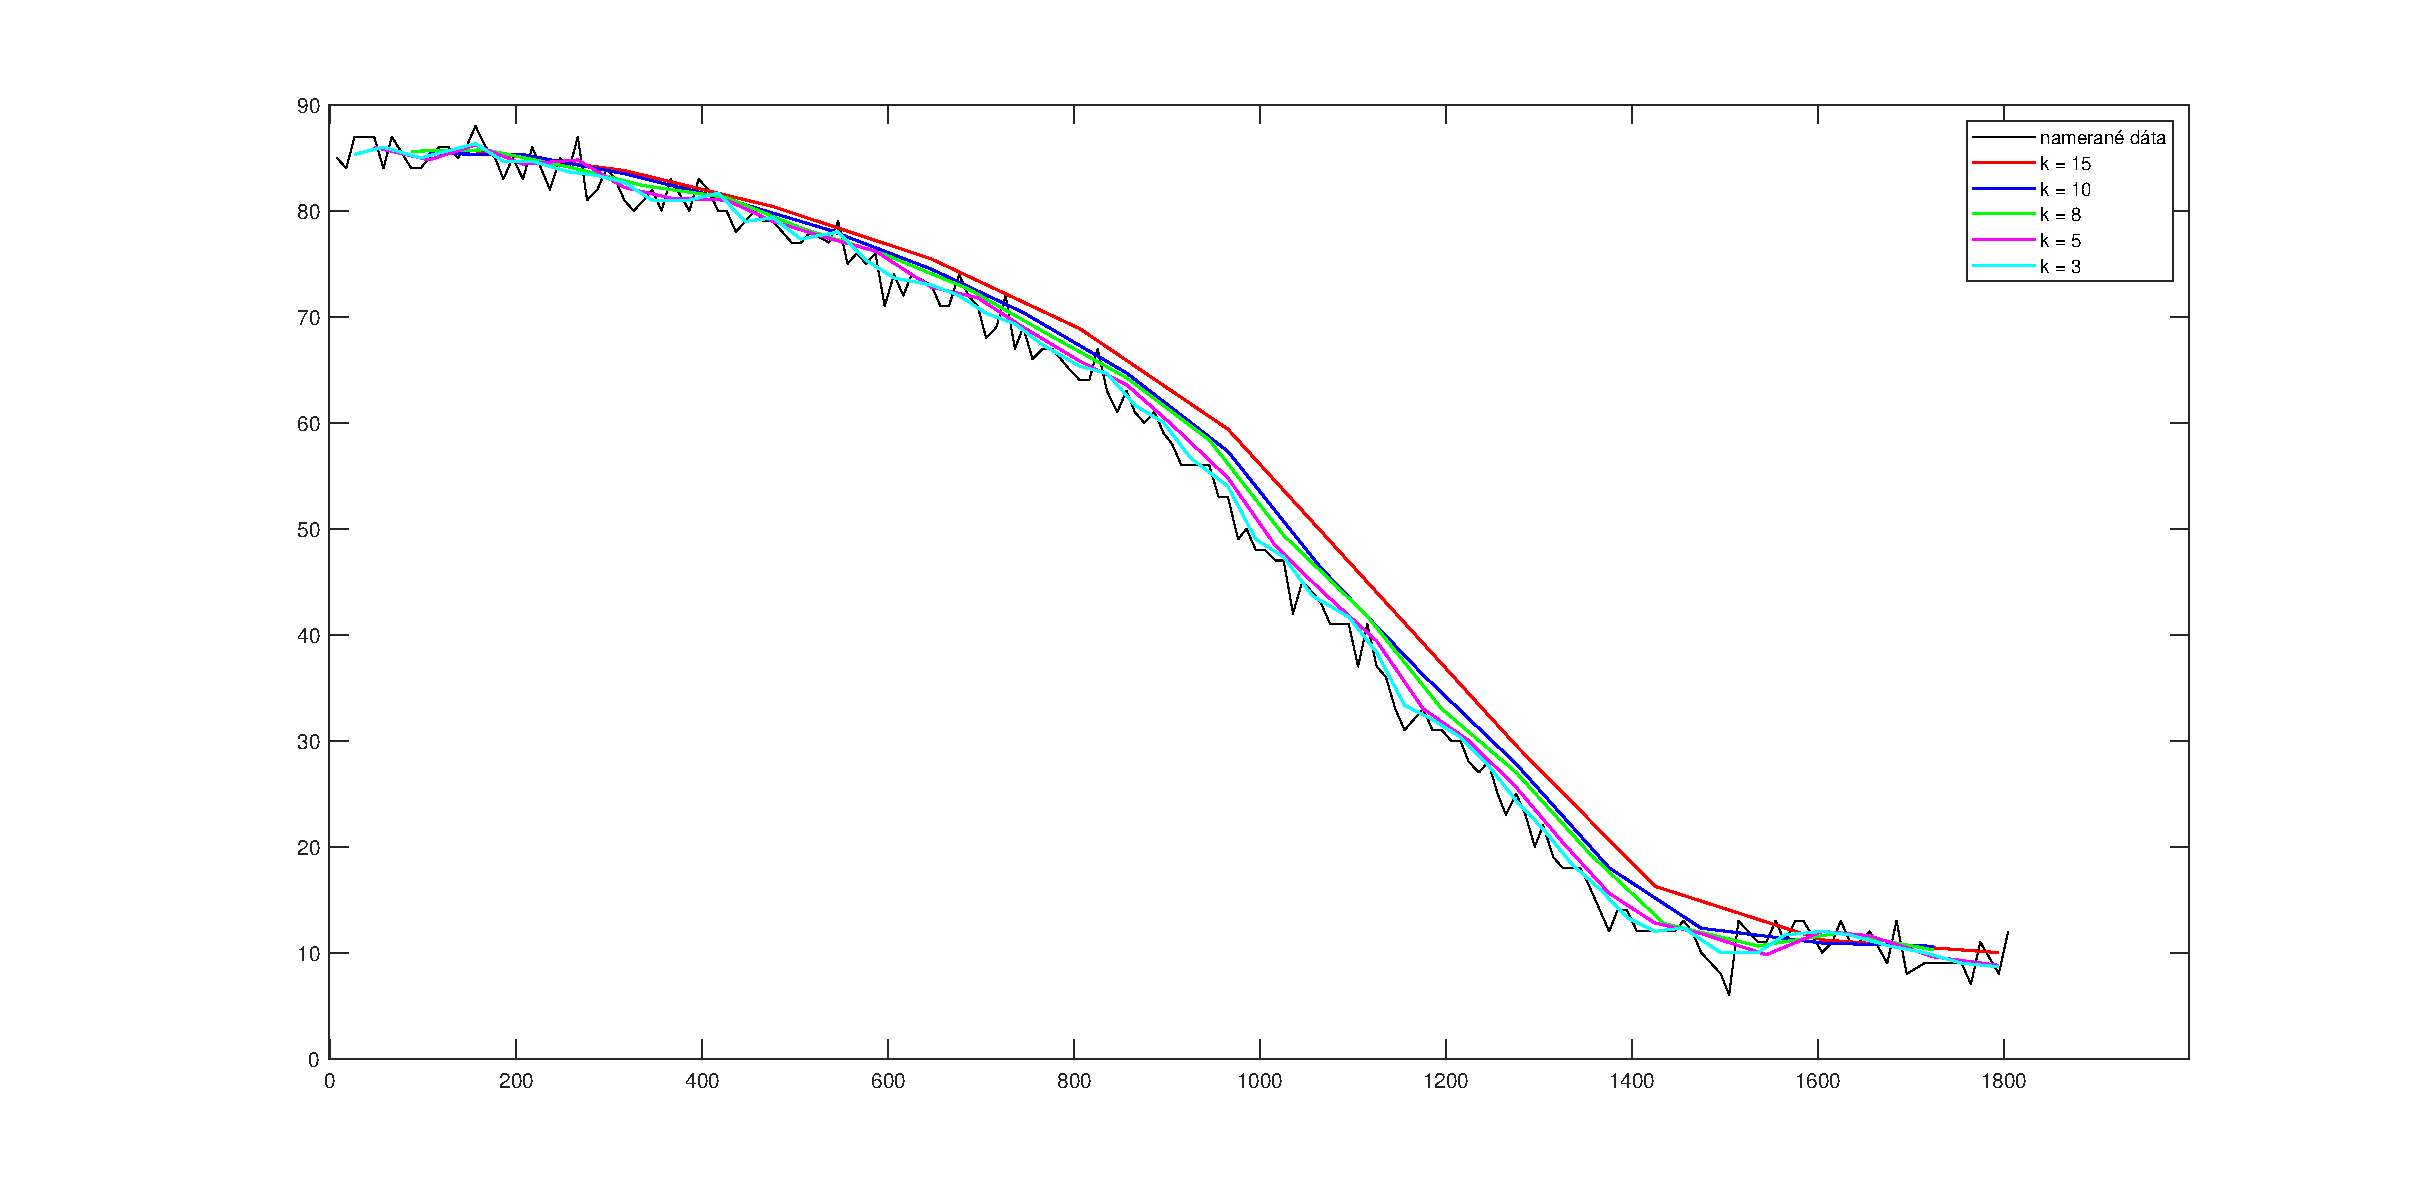
\includegraphics[width=170mm]{obr/aritmeticky.eps}
	\caption{Aritmetický priemer}\label{OBRAZOK 3.1.1.1} 
\end{figure}

Na ďalšom grafe (obr. \ref{OBRAZOK 3.1.1.2} ) môžeme vidieť filtráciu prostredníctvom plávajúceho aritmetického priemeru. Rovnako sme testovali rôzne počty hodnôt z ktorých sme daný priemer robili. Z grafu môžeme vidieť, že pri vyšších počtoch hodnôt sa krivka výrazne lepšie vyhladí, no zároveň je na grafe očividné oneskorenie oproti nefiltrovaným dátam. Z daných možností, ktoré sme testovali sme sa rozhodli pre filtráciu pomocou 5 posledných hodnôt. Krivka dobre kopíruje nefiltrované dáta z hľadiska oneskorenia a zároveň dosahuje prijateľné vyhladenie šumu.

\begin{figure}
	\centering
	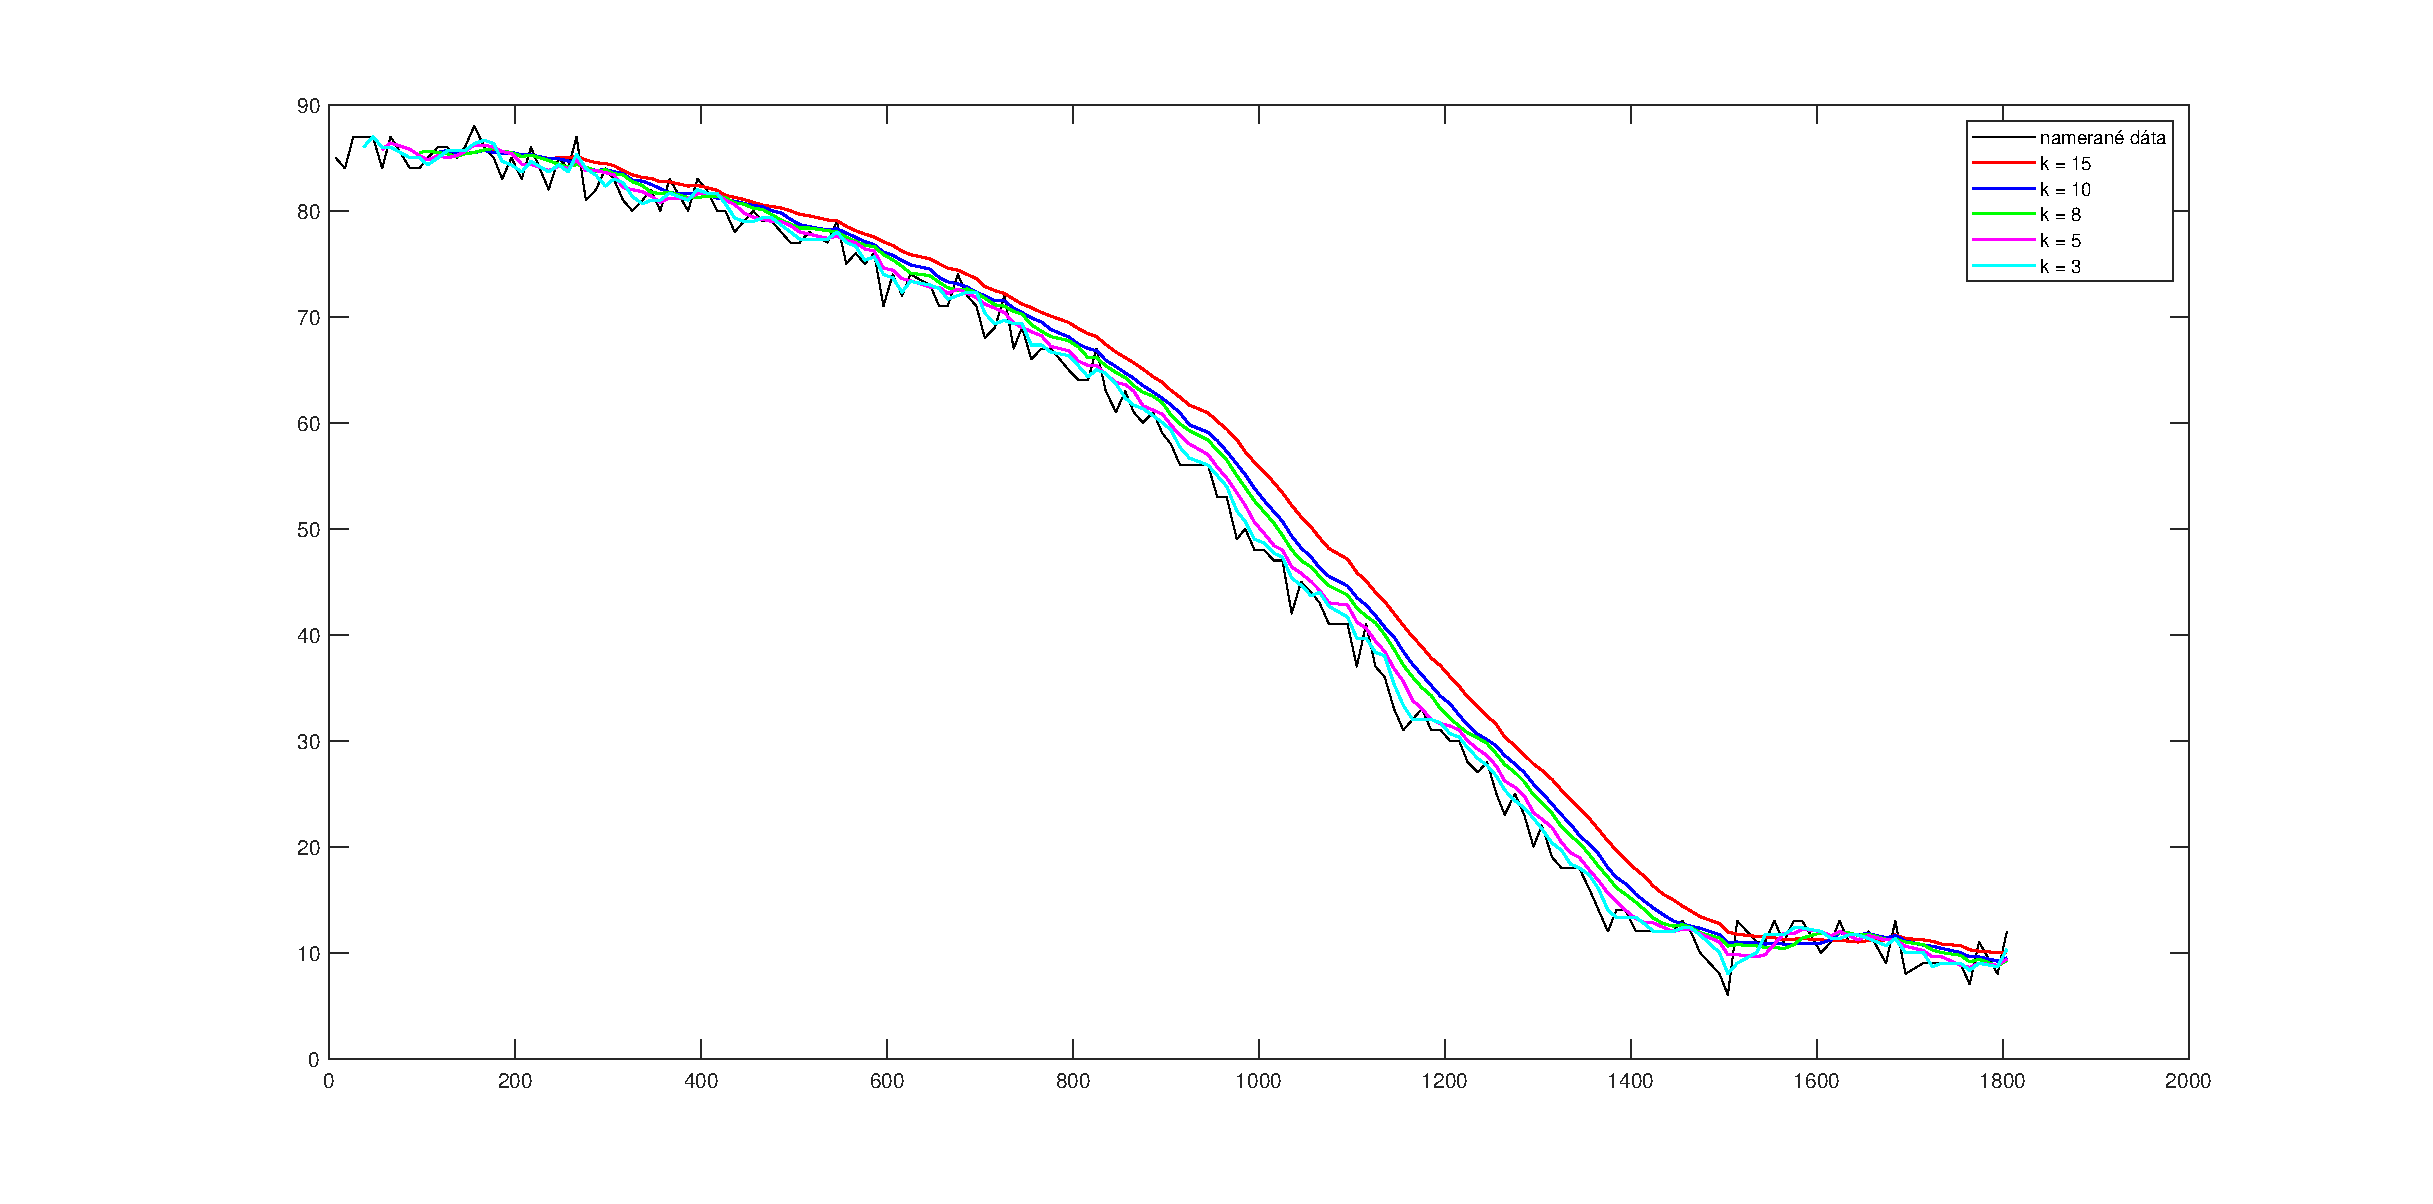
\includegraphics[width=170mm]{obr/plavajuciAritmeticky.eps}
	\caption{Plávajúci aritmetický priemer}\label{OBRAZOK 3.1.1.2} 
\end{figure}

Na grafe (obr. \ref{OBRAZOK 3.1.1.3} ) vidíme porovnanie filtrácie pomocou plávajúceho váženého priemeru z 5 hodnôt pre rozdielne faktory zabúdania. Môžeme vidieť, že rozdiel medzi jednotlivými krivkami je minimálny. Rozhodli sme sa zvoliť faktor zabúdania $\lambda = 0.4$ , keďže potrebujeme rýchlu reakciu na zmenu aktuálnej vzdialenosti, čiže dôraz na posledné hodnoty.

\begin{figure}
	\centering
	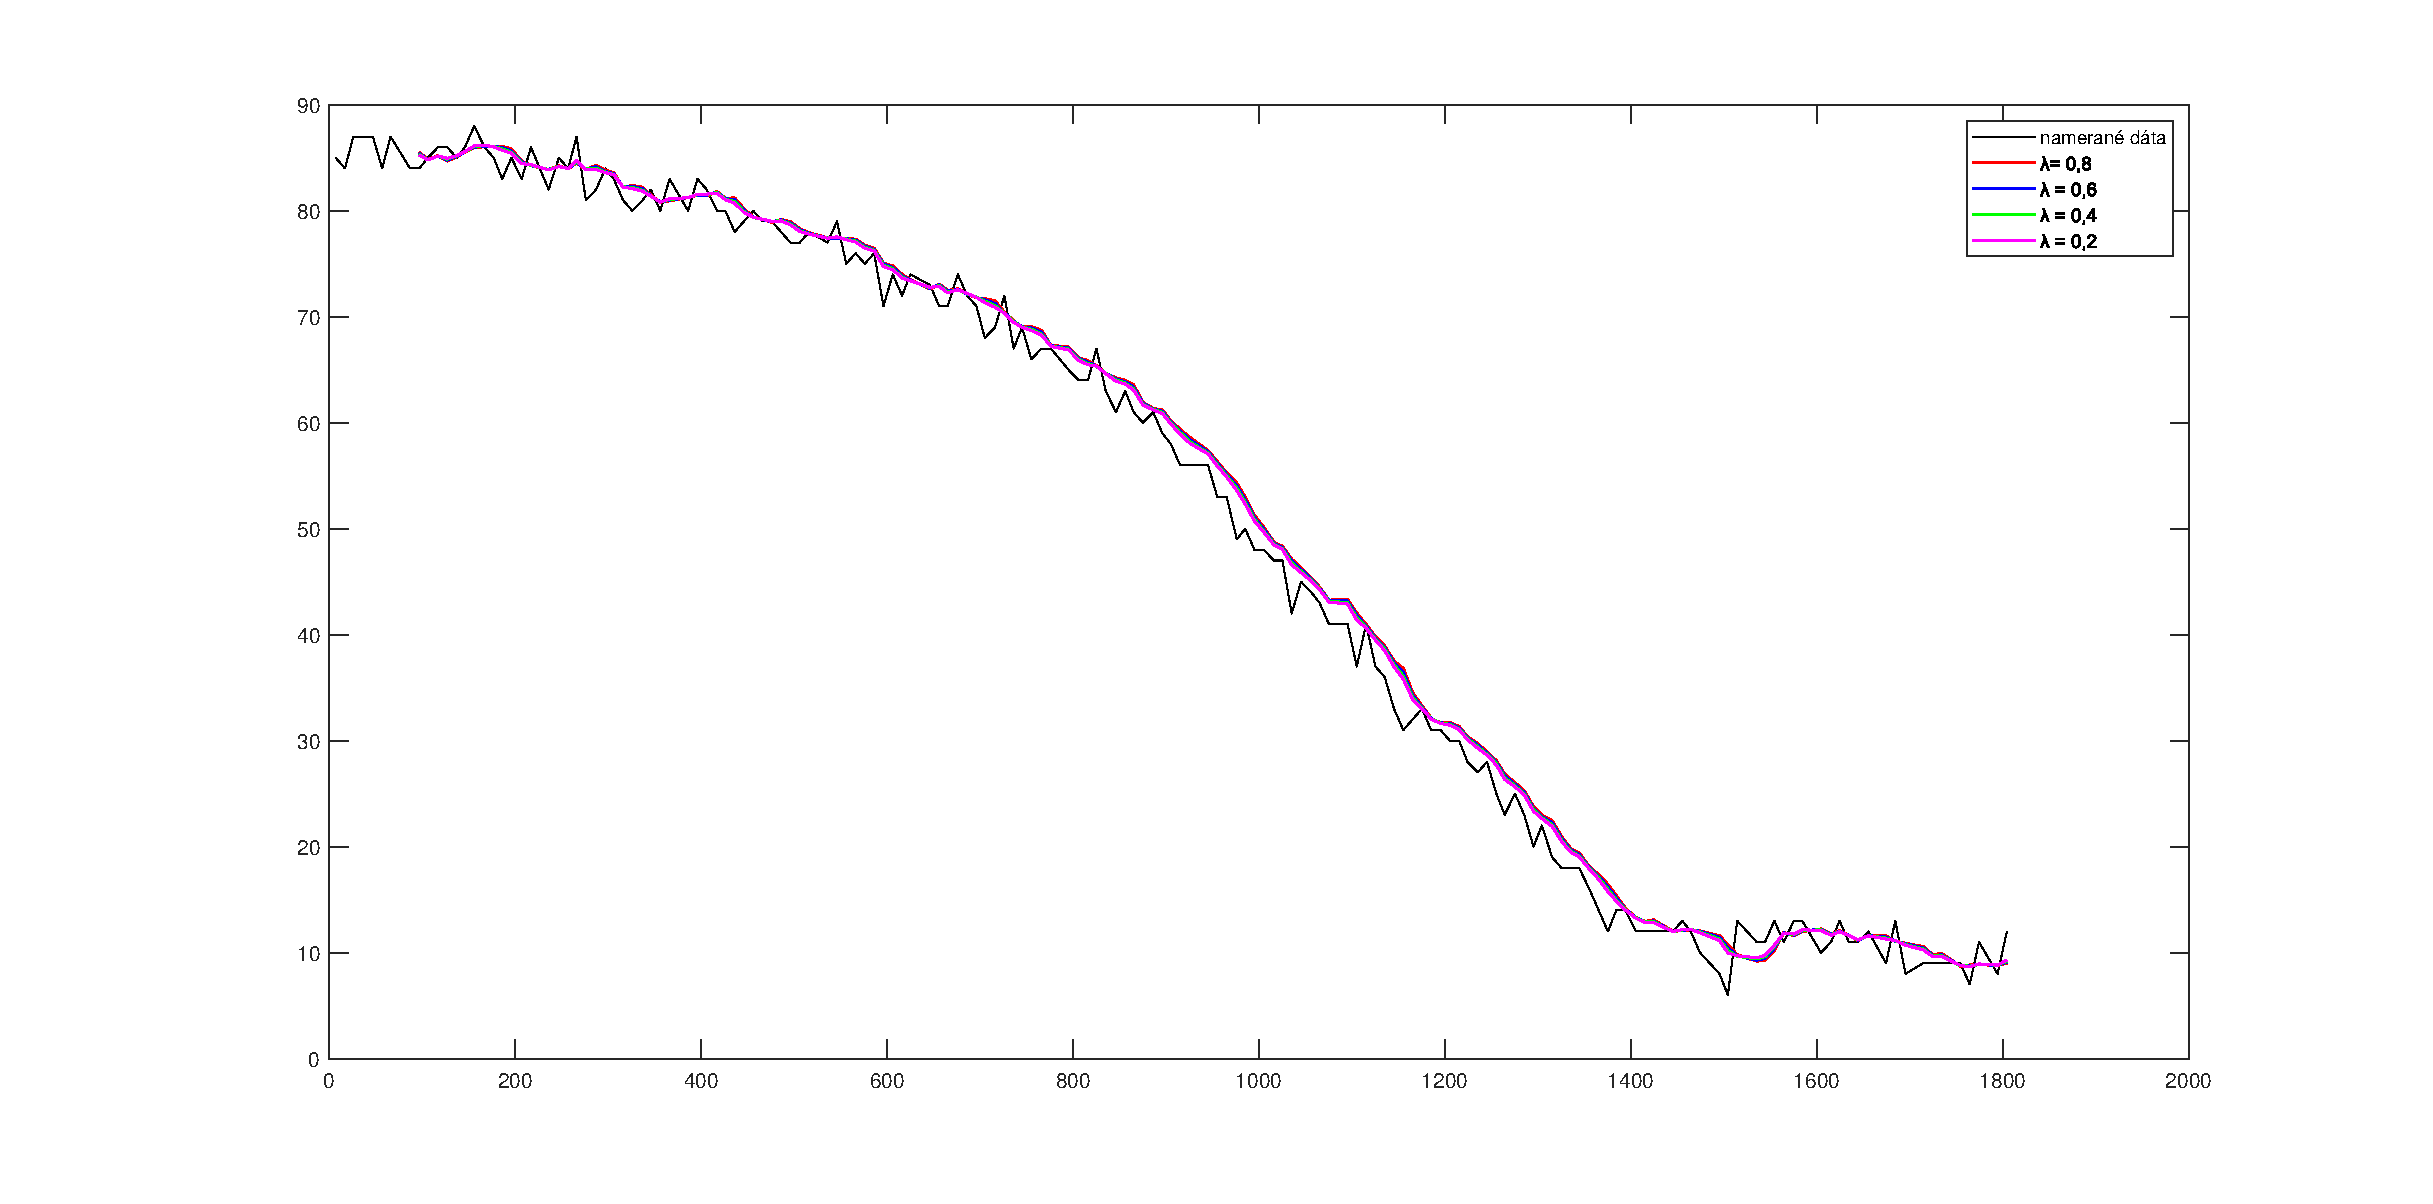
\includegraphics[width=170mm]{obr/plavajuciVazeny.eps}
	\caption{Plávajúci vážený priemer}\label{OBRAZOK 3.1.1.3} 
\end{figure}


Na obrázku \ref{OBRAZOK 3.1.1.4} môžeme vidieť porovnanie filtrácie plávajúceho aritmetického a váženého priemeru spolu s pôvodnými, nefiltrovanými nameranými hodnotami. Môžeme vidieť, že rozdiel medzi krivkami je minimálny. Jednoduchšou voľbou z hľadiska výpočtov je určite aritmetický priemer, čím budeme šetriť pamäť mikropočítača a výsledok bude takmer identický. Z tohto dôvodu sme sa rozhodli pre filtráciu pomocou plávajúceho aritmetického priemeru, počítaného z 5 posledných nameraných hodnôt.  

\begin{figure}
	\centering
	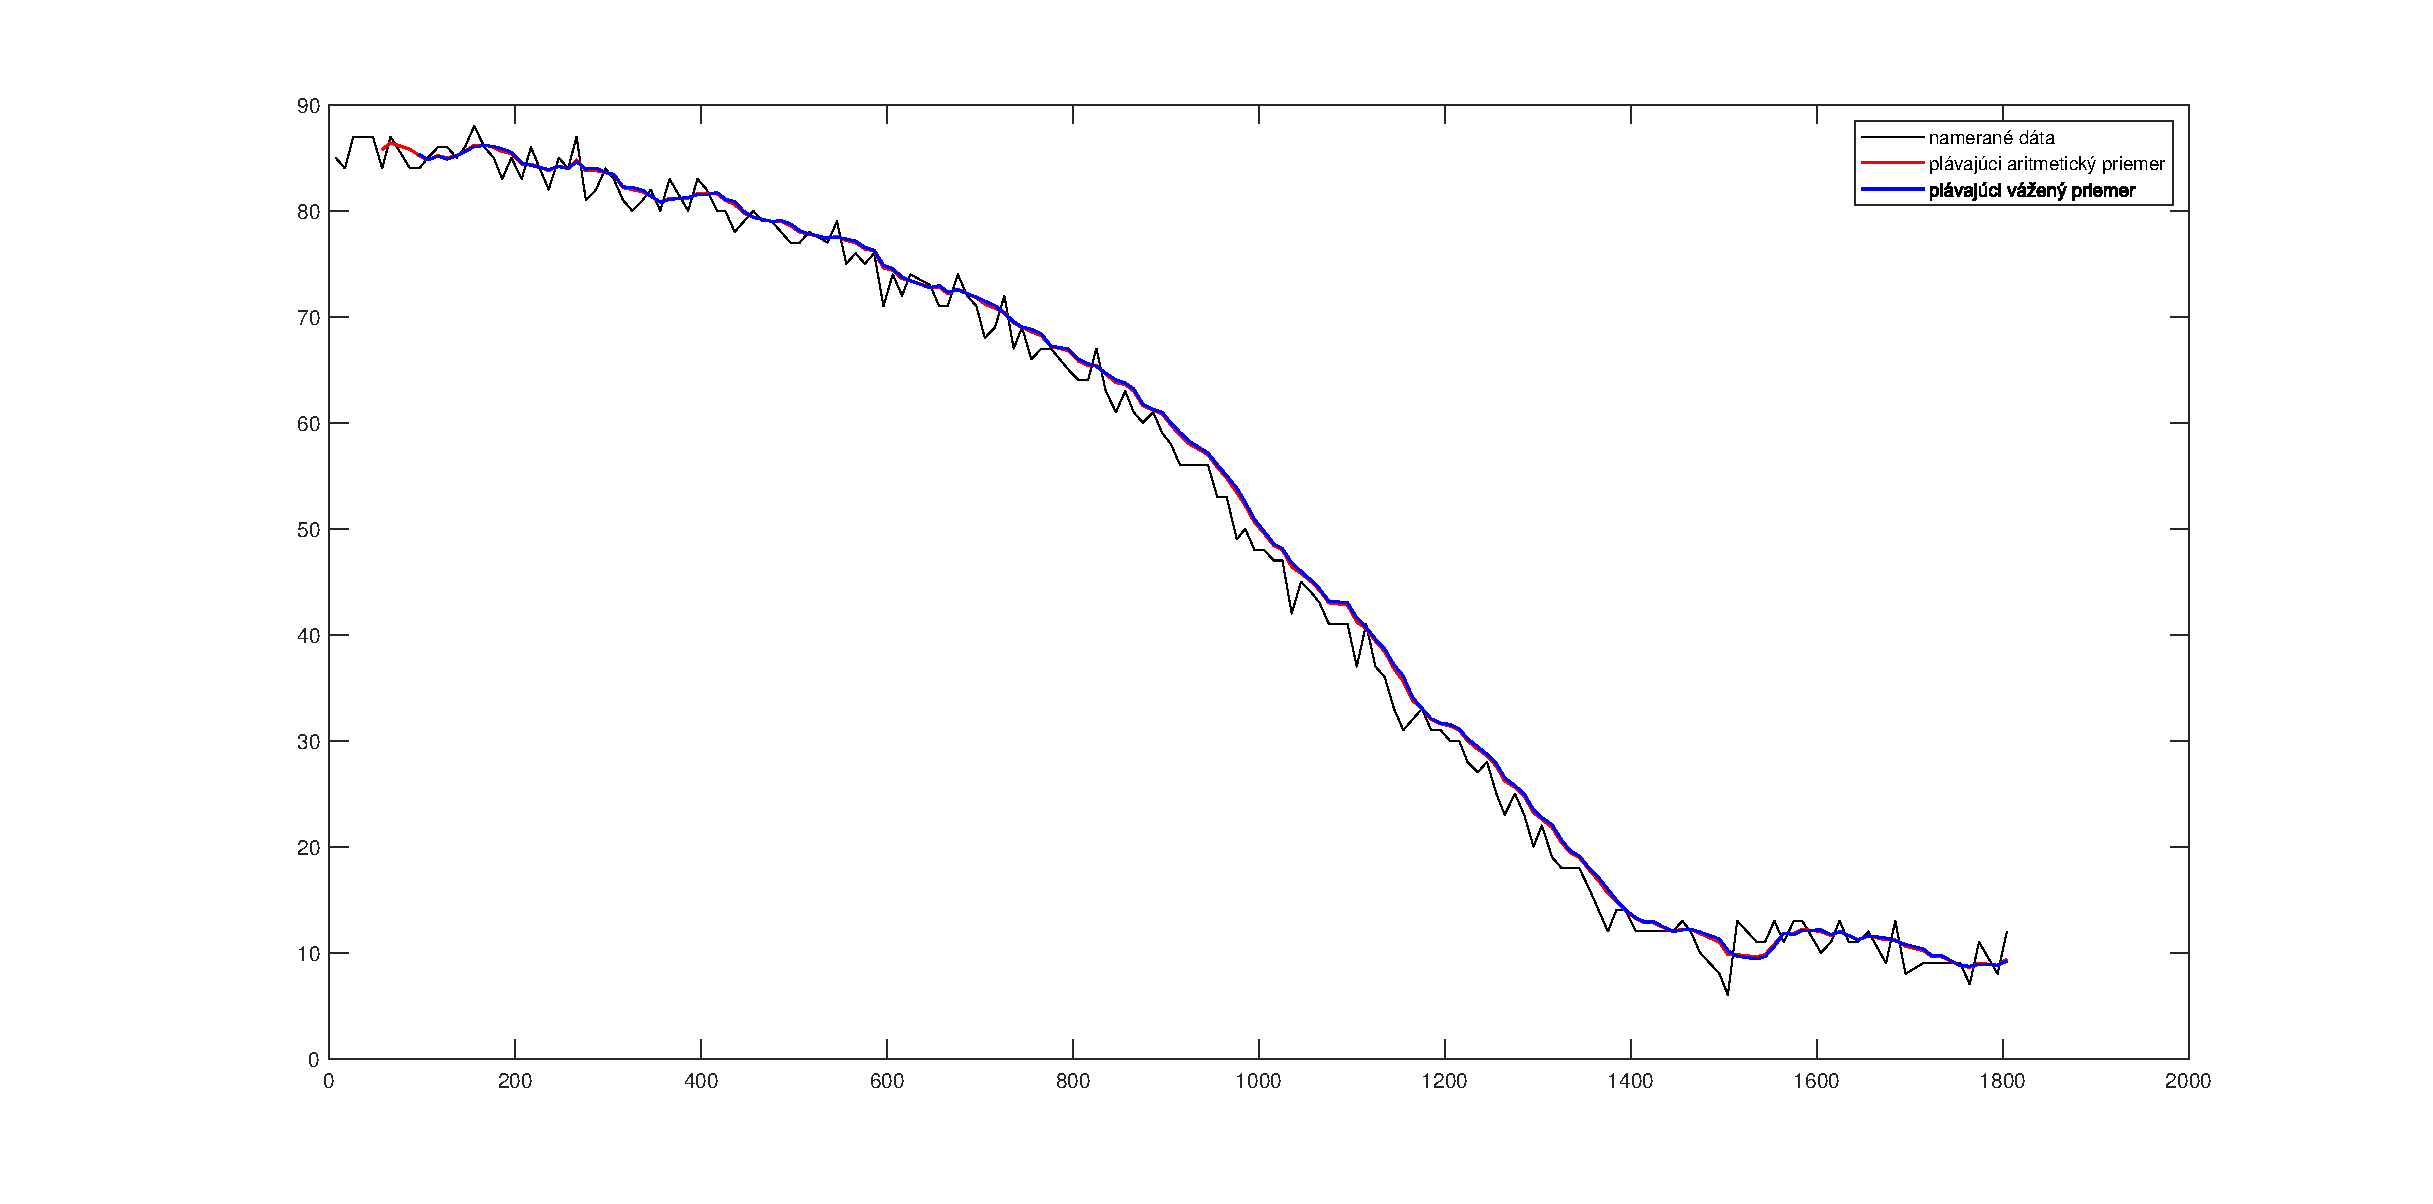
\includegraphics[width=170mm]{obr/aritmetickyVSvazeny.eps}
	\caption{Porovnanie plávajúceho artimetického a váženeého priemeru}\label{OBRAZOK 3.1.1.4} 
\end{figure}

Po výbere vhodného filtra pre odstránenie šumu sme v knižnici BOBShield.h vytvorili novú funkciu – filterSensorRead(). Jej úlohou je teda odstránenie šumu pri čítaní hodnôt zo snímača a tým zlepšiť kvalitu riadenia systému.  

\subsection{Knižnica}
\label{kap:3.1.2}

Zmeny prevedené na hardvéry sa samozrejme odrážajú aj v softvérovej časti zariadenia. Z toho dôvodu je potrebné upraviť už existujúcu knižnicu \texttt{BOBShield.h}, vytvorenú pre jednoduchú prácu so zariadením, aby bola kompatibilná aj s našou verziou zariadenia. 

Prvou vecou, ktorú sme spravili bola tvorba premennej \texttt{BOB\_SHIELD\_VERSION} definovanej na začiatku knižnice. Slúži pre nastavenie verzie zariadenia, ktorú práve používame. Momentálne v nej môžu byť nastavené 2 hodnoty a to: 2 pre verziu R2 a 3 pre verziu R3. Túto premennú využívame pri funkciách, ktorých parametre sa pre jednotlivé verzie zariadenia líšia ako je napríklad \texttt{calibration} alebo \texttt{actuatorWrite}. Jedná sa teda hlavne o funkcie, v ktorých sa nachádza nastavenie rozsahu pohybu servomotora. 

Pri funkcii \texttt{actuatorWrite}, bolo potrebné zmeniť rozsah pohybu servomotora a tiež prevod hodnôt zadávaných do funkcie na hodnoty, ktoré budú vstupovať do servomotora pri jeho riadení. Pri pôvodnej verzii išlo a jednoduchý prevod za použitia funkcie map  , kedy sa vstupné hodnoty z rozsahu -30 až 30 menili na hodnoty 65 až 125, pričom išlo a prevod celých čísel na celé čísla. 

Keďže naším cieľom bolo zlepšiť presnosť otáčania trubičky a teda zvýšiť počet hodnôt, ktoré môže nadobúdať, rozhodli sme sa pre implementáciu prevodu, v ktorom 1\degree na servomotore sa rovná 0,2\degree na trubičke. Z tohto dôvodu nie je možné využiť funkciu \texttt{map}, keďže už ide o prevod desatinných čísiel na celé. Pre prevod sme sa rozhodli použiť funkciu \texttt{mapFloat} – naprogramovanú v knižnici AutomationShield, ktorá prevádza hodnoty desatinných čísiel opäť na desatinné čísla. Teda z premennej degree, ktorá slúži na posielanie hodnôt na servomotor, sa nám stane desatinné číslo. Servomotor však dokáže pracovať len s celými číslami a preto je potrebné použiť funkciu \texttt{round()}, ktorá nám premennú degree zaokrúhli na celé číslo, ktoré už následne môžeme použiť pri riadení servomotora. Za hodnoty vstupu sme si zvolili rozsah -17 až 17 a za výstupný rozsah uhlov na servomotore 10 až 170.  

Funkcia \texttt{calibration} funguje na princípe hľadania krajných hodnôt vzdialeností guličky v trubičke pri jej pohybe. Najprv hľadá minimálnu hodnotu. Nastaví trubičku do krajnej hodnoty rozsahu jej otáčania a zmeria 100 hodnôt, z ktorých následne urobí aritmetický priemer a ten vloži do premennej minCalibrated. To isté sa deje aj pri hľadaní maximálnej hodnoty, ktorú vloží do premennej maxCalibrated. Jediné čím sa funkcia líši vo verzii R3 od pôvodnej verzie sú krajné hodnoty otočenia trubičky, tie bolo teda potrebné upraviť pre náš hardvér.


\section{API pre Simulink}
\label{kap:3.2}

Simulink je grafické programovacie prostredie založené na MATLABe a určené pre modelovanie, simuláciu a analýzu dynamických systémov.  Jeho hlavným rozhraním je nástrojom pre vytváranie grafických blokových diagramov a sada blokových knižníc, určených pre rôzne typy aplikácií. Ide o nástroj často využívaní pri automatickom riadení a využíva sa aj pri digitálnom spracovaní signálov. Táto časť práce sa venuje API vytvorenému v tomto prostredí a určenému pre riadenie nášho zariadenia. 

\subsection{Knižnica}
\label{kap:3.2.1}
Pre tvorbu rozhrania pre programovanie nášho zariadenie v prostredí Simulink je potrebné vytvoriť vlastnú knižnicu, ktorá obsahuje potrebné funkcie pre komunikáciu so zariadením.  Táto sa ale svojou formou líši od knižnice vytvorenej pre prostredie Arduino IDE. V porovnaní s ňou neobsahuje kód ako taký ale skladá sa s jednotlivých blokov, ktorých úlohou je zastrešiť určitú funkciu a následným spájaním blokov do diagramu vytvárame výsledný program, ktorý je následne pri kompilácii nahraný do mikropočítača. Knižnica je teda klasický súbor pre Simulink model ( .slx ) obsahujúci dané bloky a do zoznamu knižníc v programovacom prostredí je pridaný prostredníctvo MATLAB kódu. Aby sme knižnicu vedeli dostúpiť je potrebné spustiť súbor s názvom InstallMatlabAndSimulink nachádzajúci sa v knižnici AutomationShield. Jeho úlohou je nastaviť všetky cesty tak aby program vedel nájsť potrebné súbory pre implementáciu knižnice. Knižnica BOBShield pre Simulink už bola rozpracovaná. V našej práci sme ju sfunkčnili a doplnili o potrebné funkcie. Následne sme ju vložili medzi ostatné knižnice nachádzajúce sa AutomationShield API pre Simulink.


Jednotlivé bloky nachádzajúce sa v BOBShield knižnici teda slúžia rovnako ako funkcie naprogramované v knižnici pre Arduino IDE a zastrešujú rovnaké úlohy.

Prvým blokom je Actuator Write, ktorého úlohou je riadenie servomotora. Spracúva vstupnú hodnotu vchádzajúcu do bloku a následne nastavuje uhol otočenia servomotora v rozsahu, ktorý sme preň určili. Pri nastavovaní parametrov bloku si môžeme zvoliť typ vstupu, vchádzajúceho do bloku a to z 2 možností – v percentách a vo vzdialenosti reprezentovanej v mm.  Dôležitým parametrom je taktiež rozsah uhlov, ktorý pre blok nastavíme. Môžeme buď nechať defaultne prednastavené hodnoty v rozsahu -30\degree až +30\degree alebo zvoliť možnosť manuálneho nastavenia vlastného rozsahu kde si zvolíme minimálny a maximálny uhol otočenia.

\begin{figure}
	\centering
	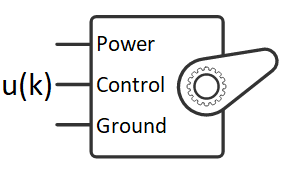
\includegraphics[width=50mm]{obr/servo.png}
	\caption{blok Actuator Write}\label{OBRAZOK 3.1.1} 
\end{figure} 

Blok Reference Read nám v diagrame reprezentuje potenciometer umiestnený na BOBShielde. Slúži na získavanie hodnôt z potenciometra, ktorý môže byť využitý ako referenčná hodnota pri riadení systému. Po kliknutí pravým tlačidlom myši na daný blok v schéme si môže užívateľ nastaviť spôsob akým budú hodnoty z potenciometra prezentované v Simulinku. Je možné zvoliť si z 3 možností, ktoré môžeme vidieť v sekcii Readout type. Prvou je získanie hodnoty v percentách, kde hodnoty, ktoré získavame, budú z intervalu od 0 po 100 v závislosti od polohy bežca potenciometra. Ďalšou možnosťou je získavanie hodnôt v podobe napätia v rozsahu od 0 po 5 V. Poslednou dostupnou možnosťou nastavenia čítania hodnôt z potenciometra je analógová hodnota z intervalu od 0 po 1023.  V závislosti od potreby užívateľa blok poskytuje teda určitú flexibilitu v závislosti od aplikácie v ktorej ho chceme využiť.

\begin{figure}
	\centering
	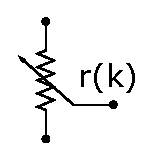
\includegraphics[width=30mm]{obr/Potentiometer.eps}
	\caption{blok Reference Read}\label{OBRAZOK 3.1.2} 
\end{figure} 

Ďalším blokom je Sensor Read a slúži nám na získavanie aktuálnej polohy guličky v trubičke. Ide o blok slúžiaci na komunikáciu mikropočítača s naším ToF snímačom VL6180X prostredníctvom I2C protokolu. Používateľ si môže vybrať z typov výstupných hodnôt zo snímača. Prvou možnosťou je vzdialenosť v mm, ktorá nám dáva vzdialenosť guličky od snímača v trubičke. Ďalšou z možnosti je pozícia guličky v mm. Ide o úpravu vzdialenosti, kde sa za počiatočnú pozíciu považuje koncový bod trubičky v ktorom sa nenachádza ToF snímač, teda výstupné hodnoty sú inverzné voči vzdialenosti. Pri voľbe výstupu v percentách sú potrebné kalibračné hodnoty aby vedel blok učiť minimálnu a maximálnu meranú hodnotu pre daný typ telesa v trubičke. Tie je možné zadať nižšie v okne parametrov bloku kedy si môžeme zvoliť buď defaultne nastavené hodnoty – 0 až 100 mm alebo nastaviť nami namerané krajné hodnoty pomocou manuálneho zadávania.

\begin{figure}
	\centering
	
\includegraphics[width=30mm]{obr/SensorRead.eps}
	\caption{blok Sensor Read}\label{OBRAZOK 3.1.3} 
\end{figure} 

Posledným blokom je blok Filtrated Sensor Read (obr. ), ktorého úlohou je vyhľadenie šumu snímača pri meraní vzdialenosti guličky. Ide o implementácia filtrácie signálu, ktorú sme si zvolili na základe testovaní viacerých typov filtrácií na nami nameranej zložke dát. Na vyhladenie šumu používame plávajúci aritmetický priemer počítaní z posledných piatich nameraných hodnôt. Daný blok sme vytvorili ako subsystém, do ktorého sme vložili blok Sensor Read a výstup z neho sme vložili do bloku Moving Averge, v ktorom sme si za veľkosť okna (parameter window length) zvolili 5 hodnôt a jeho výstup sme zaviedli na výstup zo subsystému. 


\subsection{PID príklad}
\label{kap:3.2.2}

Riadenie systému pomocou PID regulátora je jeden z najznámejších typov riadenia systému. Naše zariadenie sme sa teda rozhodli riadiť pomocou PID regulátora v uzavretej riadiacej slučke (obr.\refeq{OBRAZOK 3.2.2.1} ). V princípe sa v schéme nachádza slučka so spätnou väzbou zo zariadenia, ktorá porovnáva aktuálny stav systému s referenčnou hodnotu a na základe toho vyhodnocuje akčný zásah do systému. V našom zapojení referenčnú hodnotu dostávame z bloku Reference Read,  ktorý nám ponúka aktívne ju meniť pomocou otáčania bežcom na potenciometri. Spätnú väzbu o stave zariadenia sme získavame prostredníctvom bloku Filtered Sensor Read, ktorý nám hovorí o aktuálnej pozícii guličky v zariadení. Blok PID nám následne na základe vypočítanej chyby určí akčný zásah do systému a pošle ho do bloku Actuator Write, ktorý následne nastaví pozíciu servomotora do požadovanej hodnoty.

\begin{figure}[h]
	\centering
	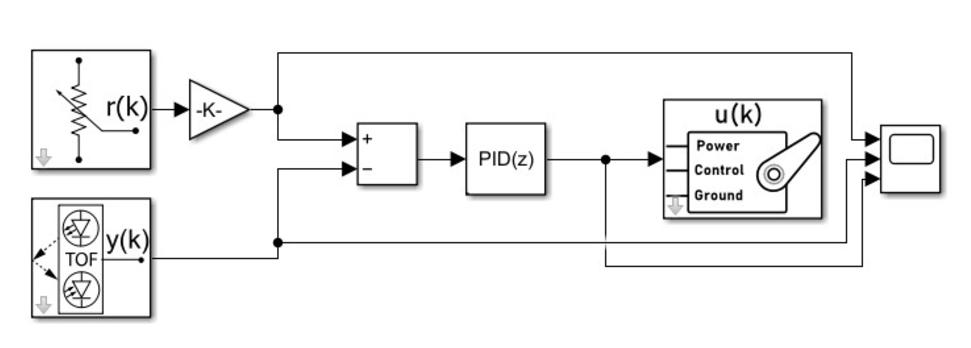
\includegraphics[width=130mm]{obr/PID.eps}
	\caption{Schéma zapojenia - príklad PID riadenia}\label{OBRAZOK 3.2.2.1} 
\end{figure} 

\begin{figure}
	\centering
	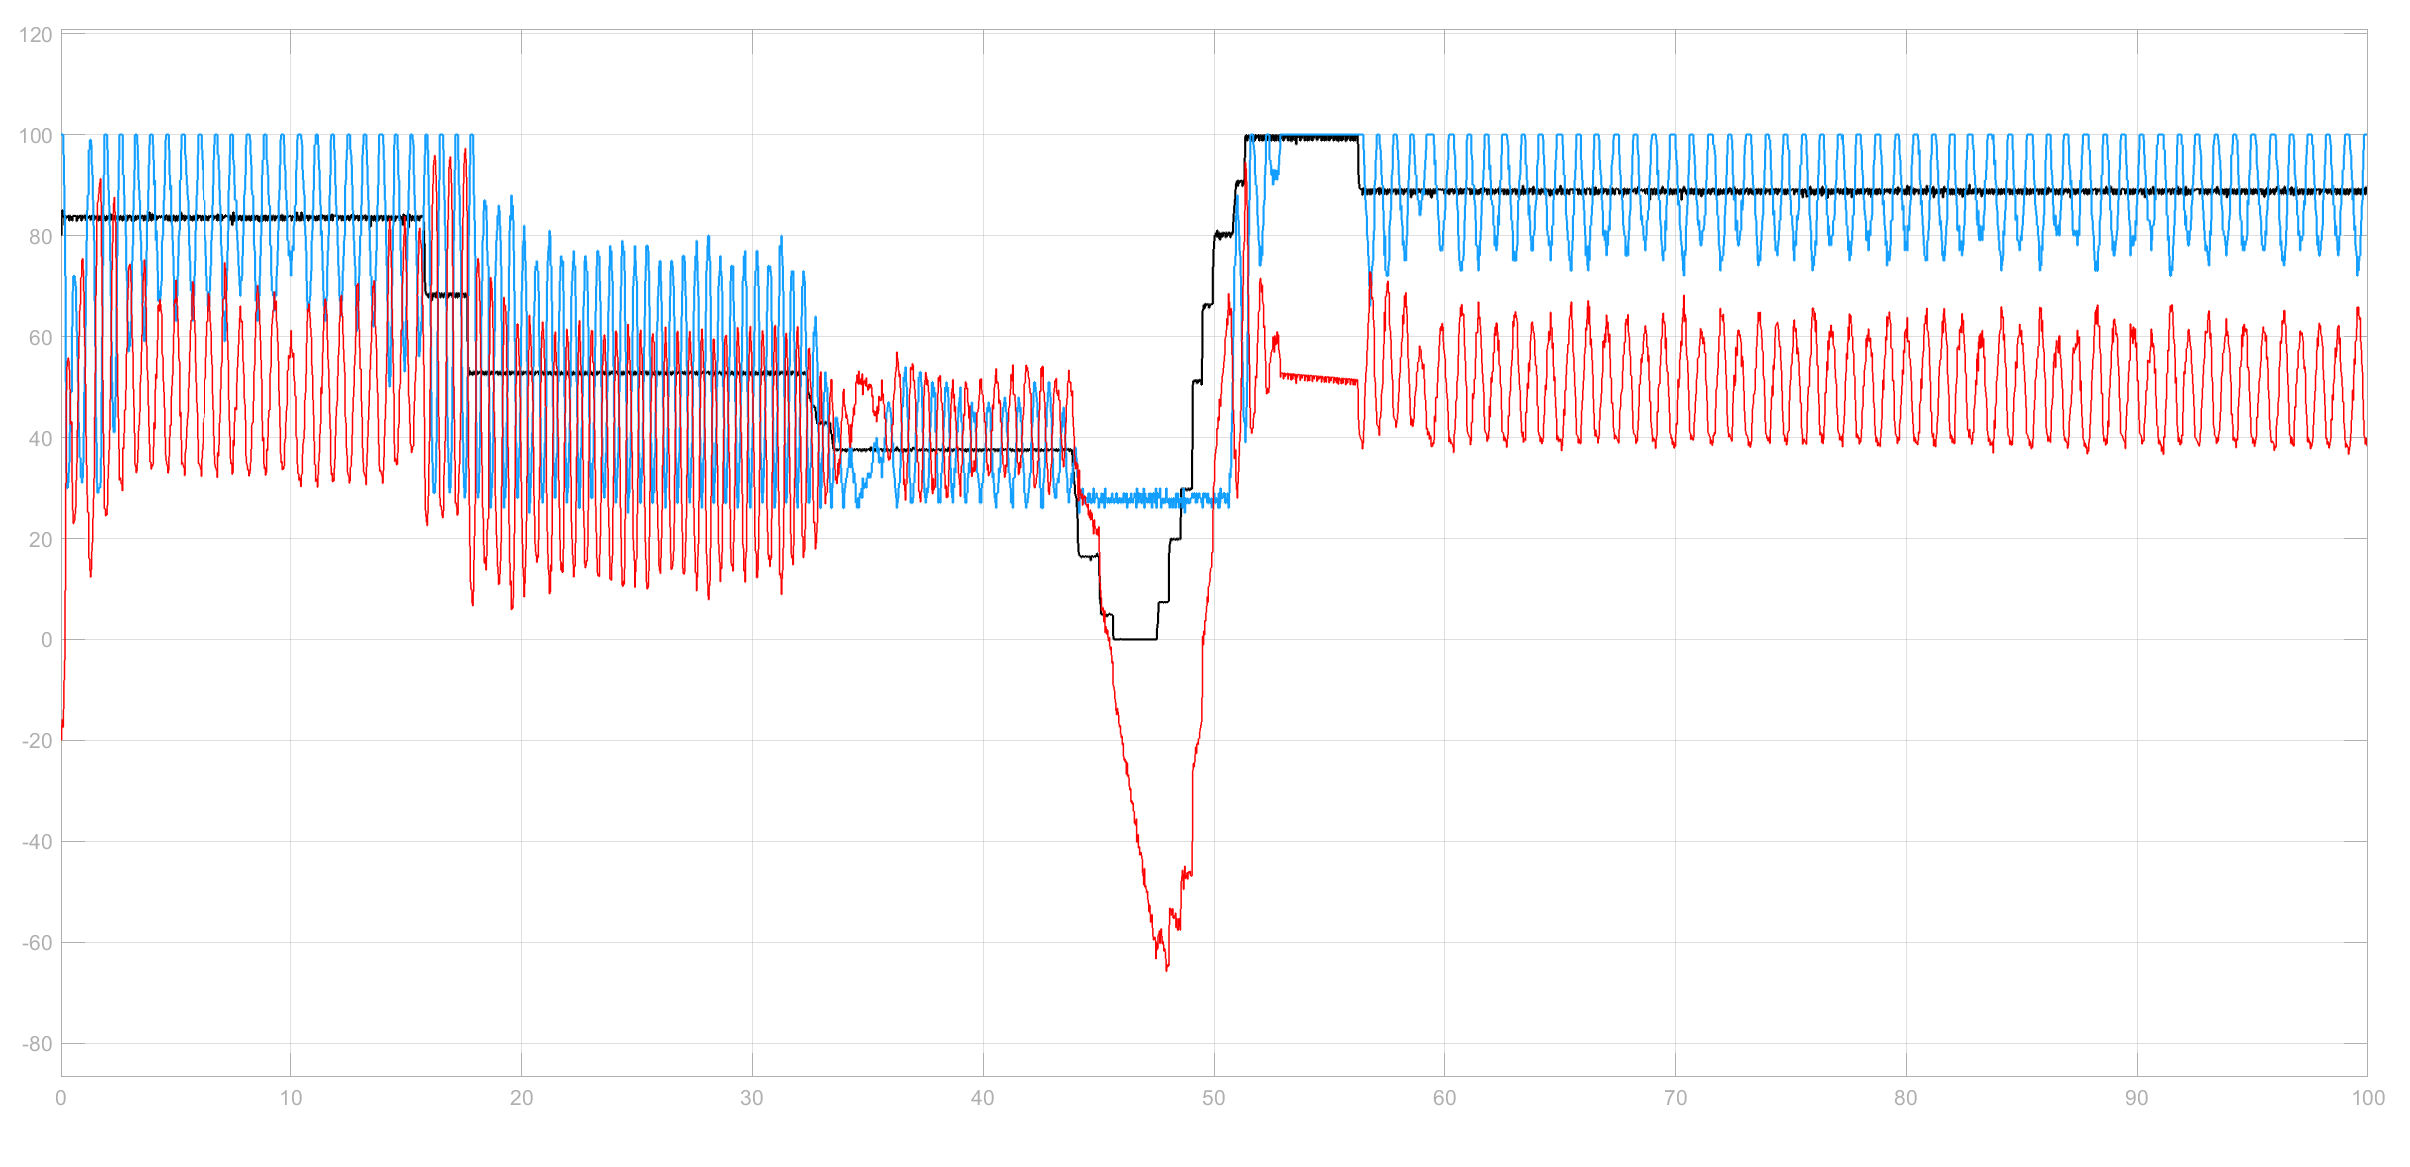
\includegraphics[width=130mm]{obr/PIDgraf.eps}
	\caption{Výstup z priebehu riadenia }\label{OBRAZOK 3.2.2.2} 
\end{figure} 
Na obrázku \refeq{OBRAZOK 3.2.2.2} môžeme vidieť výstup z priebehu riadenia, kedy krivka čiernej farby reprezentuje referenčnú hodnotu, modrá aktuálnu pozíciu guličky a červená akčný zásah do systému. Môžeme vidieť, že zariadenie na zmenu referenčnej hodnoty aktívne reaguje a snaží sa pomocou zásahu do systému regulovať polohu guličky v danej polohe. Gulička zatiaľ len osciluje okolo referenčnej polohy ale  po dôkladnom naladení by mal byť systém schopný udržať jej pozíciu priamo na požadovanej hladine. Momentálne z hľadiska problémov pri komunikácii hardvéru s rozhraním Simulink sme neboli schopný aplikovať riadny a detailný proces ladenia PID regulátora. No môžeme vidieť, že daný proces PID riadenia pomocou programu Simulink je možné uskutočniť a knižnica je plne funkčná.




	%[...]
	\chapter{Záver}

Cieľom tejto bakalárskej práce bolo zrevidovať existujúci hardvér, navrhnúť a realizovať jeho zmeny, vytvoriť API v programovacom prostredí Simulink a zrealizovať príklady riadenia systému na novom hardvéry a v novom programovacom prostredí. 

Podarilo sa nám výrazne vylepšiť hardvérovú časť zariadenie, kde sme pomocou aplikácie prevodu medzi servomotorom a trubičkou zvýšili presnosť jej otáčania z 1\degree na 0,2\degree. Tiež sme dôkladnou analýzou výberu vhodnej guličky pre náš systém znížili smerodajnú odchýlku pri meraní snímača. Z hľadiska softvéru sme pridali do pôvodnej knižnice v Arduino IDE, funkcie na filtráciu šumu a upravili sme pôvodné funkcie aby boli kompatibilné s obidvoma verziami zariadenia R2 a R3. Vytvorili sme API pre Simulink a overili jeho funkčnosť na príklade PID riadenia systému.

Taktiež sme sa snažili o tvorbu API v programovacom prostredí MATLAB, ku ktorému sme vytvorili knižnicu, no narazili sme na problém v  komunikácii medzi programovacím prostredím MATLAB a ToF snímačom, ktorý sme v našom zariadení použili. Tento problém mohol vzniknúť 

Do budúcna zariadenie stále ponúka priestor na zlepšenie. Môže dôjsť ku tvorbe nových príkladov LQ riadenia pre obe API, taktiež ku procesu identifikácie systému na novom hardvéry. Taktiež ku tvorbe funkcie na nastavenie vodorovnej polohy trubičky pri kalibrácii systému, ktorá nemohla byť vytvorená z dôvodu nedodanie komponentov na jej realizáciu.


	
	%%%%%%% Koniec %%%%%%%%
	\bibliographystyle{abbrv}
	\addcontentsline{toc}{chapter}{Literat\'{u}ra}
	\bibliography{bibliog.bib}
	
	\begin{thebibliography}{10}
	\bibitem{VL6180X}
	\textbf{STMicroelectronics}, \textit{VL6180X - Proximity and ambient light sensing module} [online], 2016, [cit 2022-4-21] Dostupné z: \url{https://www.st.com/resource/en/datasheet/vl6180x.pdf } 
	
	\bibitem{MPU6050}
	\textbf{InvenSense Inc.}, \textit{MPU-6000 and MPU-6050 Product Specification Revision 3.4} [online], 2013 [cit. 2022-4-21] Dostupné z:
	\url{https://invensense.tdk.com/wp-content/uploads/2015/02/MPU-6000-Datasheet1.pdf}
	
	\bibitem{LDO}
	\textbf{STMicroelectronics}, \textit{ST732 Datasheet} [online], 2021 [cit. 2022-4-28] Dostupné z:
	\url{https://www.mouser.sk/ProductDetail/STMicroelectronics/ST732M28R?qs=MLItCLRbWsxtXiiWQqtIMw%3D%3D}
	
	\bibitem{Anicka}
	\textbf{A. Vargová}, \textit{BoBShield: a miniature "ball on beam" experiment}, Slovenská technická univerzita v Bratislave, Strojnícka fakulta, 2021, Bratislava, Slovenská republika
	
	
	\bibitem{BOBexperiment}
	\textbf{CTMS - Control tutorials for MATLAB and SIMULINK}, \textit{Ball and Beam: System Modeling} [online], [cit. 2022-5-12] Dostupné z:
	\url{https://github.com/gergelytakacs/AutomationShield/wiki/BoBShield}
	
	
	\bibitem{Autoshield}
	\textbf{G. Takacs}, \textit{BOBShield} [online], [cit. 2022-4-22] Dostupné z:
	\url{https://www.hennlich.sk/fileadmin/user_upload/sk_gufer%C3%A1_-_preh%C4%BEad_profilov.pdf}
	
	
	\bibitem{Servo}
	\textbf{ISL Products International Ltd.}, \textit{Servo Motor Fundamentals} [online]. [cit. 2022-5-20] Dostupné z:
	\url{https://islproducts.com/design-note/servo-motor-fundamentals/}
	
	\bibitem{Servo-stare}
	\textbf{DFROBOT}, \textit{9g Metal Gear Micro Servo (1,8Kg)} [online]. [cit. 2022-4-22] Dostupné z:
	\url{https://www.dfrobot.com/product-1338.html}
	
	\bibitem{Servo-nove}
	\textbf{SAVOX-SERVO}, \textit{Savox - Servo - SH-0253 - Digital - DC - Motor } [online]. [cit. 2022-5-22] Dostupné z:
	\url{https://www.savox-servo.com/Servos-c-1338/Brushed-Motor-c-1340/Savox-Servo-SH-0253-Digital-DC-Motor/}
	
	
	\bibitem{MPUfoto}
	\textbf{MOUSER Electronics}, \textit{MPU-6050} [online]. [cit. 2022-5-12] Dostupné z:
	\url{https://www.mouser.sk/ProductDetail/TDK-InvenSense/MPU-6050?qs=u4fy%2FsgLU9O14B5JgyQFvg%3D%3D}
	
	\bibitem{Priemer}
	\textbf{MathWorks}, \textit{Sliding Window Method and Exponetial Weigthing Method} [online]. [cit. 2022-5-22] Dostupné z:
	\url{https://www.mathworks.com/help/dsp/ug/sliding-window-method-and-exponential-weighting-method.html}
	
	
\end{thebibliography}
\end{document}